\documentclass[tikz,border=8pt]{standalone}
% Shared look for every TikZ diagram. Load with % Shared look for every TikZ diagram. Load with % Shared look for every TikZ diagram. Load with \input{../../tools/tikz-style.tex}
\usepackage[T1]{fontenc}
\usepackage{lmodern}
\renewcommand{\sfdefault}{lmr}  % diagrams use the same serif as the text
\usetikzlibrary{arrows.meta, positioning, shapes.geometric, calc, fit, backgrounds}
\definecolor{cblue}{HTML}{4C78A8}
\definecolor{corange}{HTML}{F58518}
\definecolor{cgreen}{HTML}{54A24B}
\definecolor{cred}{HTML}{E45756}
\definecolor{cpurple}{HTML}{B279A2}
\definecolor{cgrey}{HTML}{6B6B6B}
\tikzset{
  every picture/.style={font=\sffamily, line width=1.2pt},
  box/.style={draw=#1, fill=#1!12, rounded corners=4pt, align=center, inner sep=7pt, minimum height=1.1cm},
  box/.default=cgrey,
  arrow/.style={-{Stealth[length=3mm]}, draw=cgrey, line width=1.4pt},
  title/.style={font=\sffamily\bfseries\Large},
  note/.style={font=\sffamily\small, text=cgrey, align=center},
}
\AtBeginDocument{\hyphenpenalty=10000 \exhyphenpenalty=10000}

\usepackage[T1]{fontenc}
\usepackage{lmodern}
\renewcommand{\sfdefault}{lmr}  % diagrams use the same serif as the text
\usetikzlibrary{arrows.meta, positioning, shapes.geometric, calc, fit, backgrounds}
\definecolor{cblue}{HTML}{4C78A8}
\definecolor{corange}{HTML}{F58518}
\definecolor{cgreen}{HTML}{54A24B}
\definecolor{cred}{HTML}{E45756}
\definecolor{cpurple}{HTML}{B279A2}
\definecolor{cgrey}{HTML}{6B6B6B}
\tikzset{
  every picture/.style={font=\sffamily, line width=1.2pt},
  box/.style={draw=#1, fill=#1!12, rounded corners=4pt, align=center, inner sep=7pt, minimum height=1.1cm},
  box/.default=cgrey,
  arrow/.style={-{Stealth[length=3mm]}, draw=cgrey, line width=1.4pt},
  title/.style={font=\sffamily\bfseries\Large},
  note/.style={font=\sffamily\small, text=cgrey, align=center},
}
\AtBeginDocument{\hyphenpenalty=10000 \exhyphenpenalty=10000}

\usepackage[T1]{fontenc}
\usepackage{lmodern}
\renewcommand{\sfdefault}{lmr}  % diagrams use the same serif as the text
\usetikzlibrary{arrows.meta, positioning, shapes.geometric, calc, fit, backgrounds}
\definecolor{cblue}{HTML}{4C78A8}
\definecolor{corange}{HTML}{F58518}
\definecolor{cgreen}{HTML}{54A24B}
\definecolor{cred}{HTML}{E45756}
\definecolor{cpurple}{HTML}{B279A2}
\definecolor{cgrey}{HTML}{6B6B6B}
\tikzset{
  every picture/.style={font=\sffamily, line width=1.2pt},
  box/.style={draw=#1, fill=#1!12, rounded corners=4pt, align=center, inner sep=7pt, minimum height=1.1cm},
  box/.default=cgrey,
  arrow/.style={-{Stealth[length=3mm]}, draw=cgrey, line width=1.4pt},
  title/.style={font=\sffamily\bfseries\Large},
  note/.style={font=\sffamily\small, text=cgrey, align=center},
}
\AtBeginDocument{\hyphenpenalty=10000 \exhyphenpenalty=10000}

\begin{document}
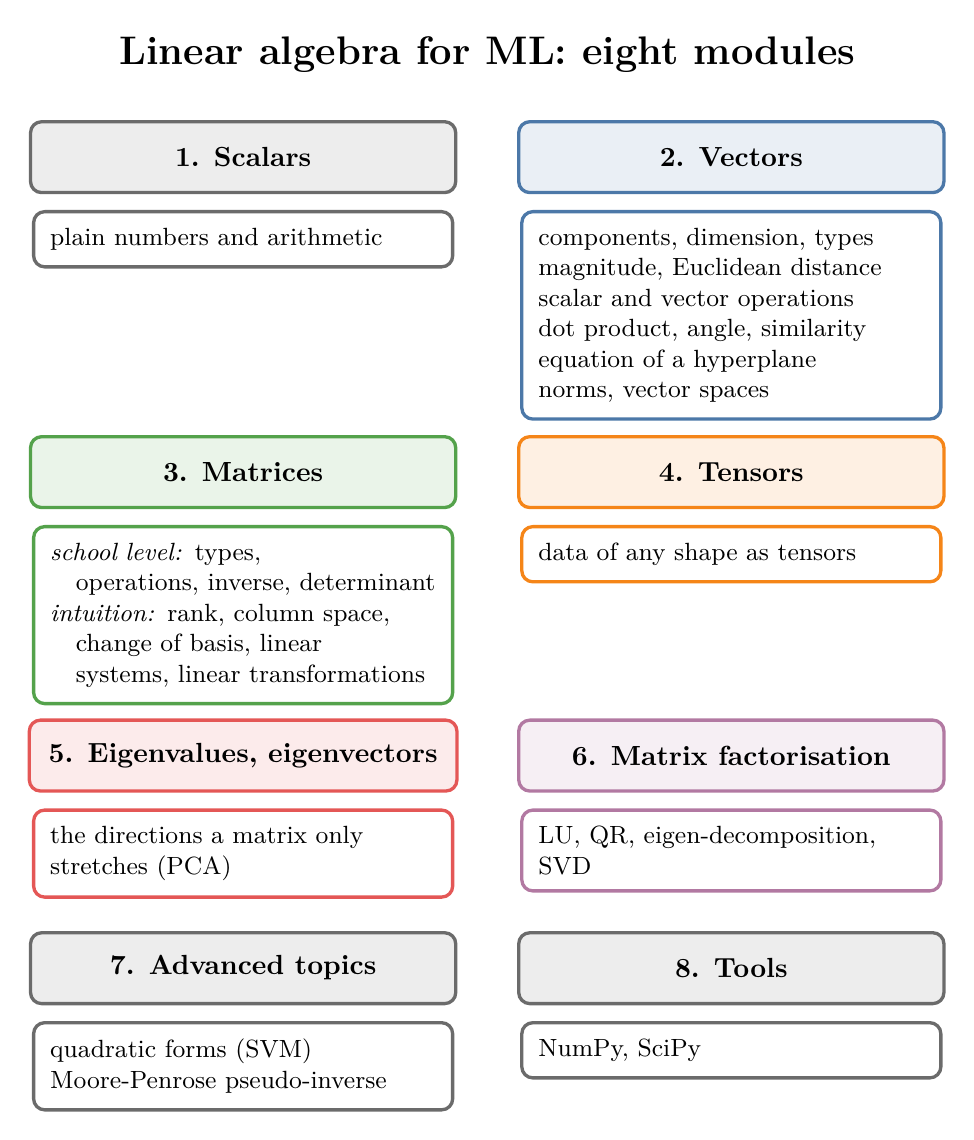
\begin{tikzpicture}[
  mod/.style={box=#1, font=\sffamily\bfseries, minimum width=5.4cm, minimum height=0.9cm},
  topics/.style={draw=#1, fill=white, rounded corners=4pt, align=left, inner sep=6pt, text width=4.9cm, font=\sffamily\small},
]
  \node[title] at (3.1,1.3) {Linear algebra for ML: eight modules};

  \node[mod=cgrey] (s) at (0,0) {1. Scalars};
  \node[topics=cgrey, below=0.2cm of s] (st) {plain numbers and arithmetic};

  \node[mod=cblue] (v) at (6.2,0) {2. Vectors};
  \node[topics=cblue, below=0.2cm of v] (vt) {components, dimension, types\\ magnitude, Euclidean distance\\ scalar and vector operations\\ dot product, angle, similarity\\ equation of a hyperplane\\ norms, vector spaces};

  \node[mod=cgreen] (m) at (0,-4.0) {3. Matrices};
  \node[topics=cgreen, below=0.2cm of m] (mt) {\textit{school level:} types,\\ \quad operations, inverse, determinant\\ \textit{intuition:} rank, column space,\\ \quad change of basis, linear\\ \quad systems, linear transformations};

  \node[mod=corange] (t) at (6.2,-4.0) {4. Tensors};
  \node[topics=corange, below=0.2cm of t] (tt) {data of any shape as tensors};

  \node[mod=cred] (e) at (0,-7.6) {5. Eigenvalues, eigenvectors};
  \node[topics=cred, below=0.2cm of e] (et) {the directions a matrix only\\ stretches (PCA)};

  \node[mod=cpurple] (f) at (6.2,-7.6) {6. Matrix factorisation};
  \node[topics=cpurple, below=0.2cm of f] (ft) {LU, QR, eigen-decomposition,\\ SVD};

  \node[mod=cgrey] (a) at (0,-10.3) {7. Advanced topics};
  \node[topics=cgrey, below=0.2cm of a] (at) {quadratic forms (SVM)\\ Moore-Penrose pseudo-inverse};

  \node[mod=cgrey] (l) at (6.2,-10.3) {8. Tools};
  \node[topics=cgrey, below=0.2cm of l] (lt) {NumPy, SciPy};
\end{tikzpicture}
\end{document}
